\section{Software Choice}
The hardware choice and implementation includes a software that can handle them. The software choice will be explained in this section, describing the use if the Kernel, and the principle of scheduling.

\subsection{Kernel}
The chosen kernel allows to control the tasks and then the behavior of the vehicle through clocks, to have a precise and constant schedule. This propriety make possible to export it on another kind of processor and still have the same render, as long as it have a frequency high enough to process all the data needed.\\
The Kernel advantage is also the definition of semaphores, priorities, and critical regions, that the system will use to choose which task to run, and how often it should be. This Kernel allows also to program in Arduino language which is C++, and can run C code.

\subsection{Scheduling}\label{sec:scheduling}
For running the code on the arduino PCB, and be able to manage all the sensors at the same time, a scheduling is needed. Indeed, the PCB must be able to recieve and process the data from the GoT system, the hall sensors, the magnetometer and the X-bee to make a decision related to the planned route to follow. This decision must affect at the same time the speed through the motor, and the steering through the servo.
A description of the scheduling principle and its function will be described.

\subsubsection{Semaphores}
In programming, a semaphore is an variable or abstract data that is used to prioritize the different tasks to use. It allows a multiprogramming, with functions that use different ressources and time, and does not interact with each others direcly. Running them independently ease the indent of the code.

\subsubsection{Tasks}
The different functions of the vehicle have been separated into multiple tasks, that can switch regarding to their priority. Five tasks are created to control the vehicle:

\begin{lstlisting} [caption = {Implementation of the tasks}, label = {lst:tasks}]

  task1 = k_crt_task(tSpeed, 10, stack, 300);         		// Hall Sensors
  task2 = k_crt_task(SpeedControl, 12, stack2, 300); 		// Velocity controller
  task3 = k_crt_task(SteeringControl, 11, stack3, 1000); 	// Angular controller(Inner loop of the steering model)
  task4 = k_crt_task(LeadCompensator, 13, stack4, 300); 	// Distance Control(Outer loop of the steering model)
  task5 = k_crt_task(GoT,14,stack5,1000);        		    // GoT and protocol handling

\end{lstlisting}

Those declarations of the tasks are made thanks to the function k\_crt\_task needing the name of the function to run, it's priority, the area to use and it's lenght. The implementation of this function can be seen below.


\begin{lstlisting} [caption = {Declaration of the tasks}, label = {lst:tasks}]

 struct k_t *k_crt_task (void (*pTask) (void), char prio, char *pStk, int stkSize);
 
\end{lstlisting}

\textbf{Hall Sensors:}
The two hall sensors of the two belts are read at a certain frequency, and knowing the distance the vehicle moves during a full turn of the drive wheel, the real speed can be calculated independently from each other belts.

\textbf{Angular Control:}
The steering task is gets the reading from the magnetometer, transform them in the coordinate system that fit the model. Then those values are converted into a heading angle, that will be used in the steering P-Controller to calculate the new angle to follow from the angle wanted. The decision will be sent directly to the servo. This is the inner loop from the Steering Model, seen in \secref{steeringModel}

\textbf{Speed Control:}
A wanted speed value is compared to the actual speed, and the resulting error is the input of the Velocity PI-Controller, that will set a new speed according to the reference.

\textbf{Distance control:}
If the angular control is in charge of the direction wanted, it can not control the position from the line wanted to be on. The task Distance Control calculate the distance of the vehicle from the line it should follow, and calculate a new heading for the angular control to follow to get back on the line. This is the outer loop from the Steering Model, seen in \secref{steeringModel}.

\textbf{GoT System and Communication Protocol:}
This task is the communication protocol handling, that receive on the vehicle the position that the GoT system sended. It will receive data from the computer, and convert it into a position so that the distance control can calulate the new heading to follow.


\subsubsection{Queue}
The tasks are meant to be done at the time they are told to be done, ensuring the good control of the vehicle. But some functionnalities are not critical, and can wait until the processor have time to do them.\\
To get a list of things to do until one of them become critical, the tasks will be stored in a queue, that will execute them one after the other, until a critical task shortcut them. The order of the task will be done regarding their priorities.


\subsubsection{Round Robin Schedule}
A way of calculating the minimum time needed to execute all the tasks in a period of time, is by putting them one after the other, and see if the sum of the time necessary to execute all the task is bigger than the time allowed to do one full turn of the tasks.

A picture illustrating the round robin schedule can be seen in \figref{roundRobinSchedule}\\

 \begin{figure}[H]
	\centering
	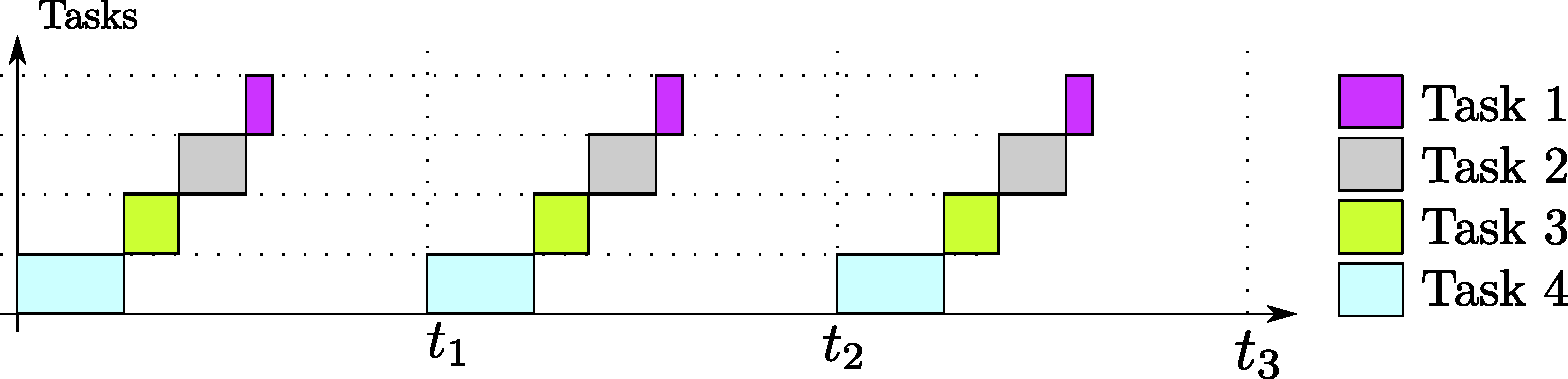
\includegraphics[scale=0.5]{figures/roundRobinSchedule.pdf}
	\caption{An example of the use of round robien schedule}
	\label{roundRobinSchedule}
\end{figure}

If the time allowed by the frequency sampling of the program is not large enough, the data will be prioritized and run in the time allowed. An example of this case can be seen on \figref{roundRobinSchedule2}.

 \begin{figure}[H]
	\centering
	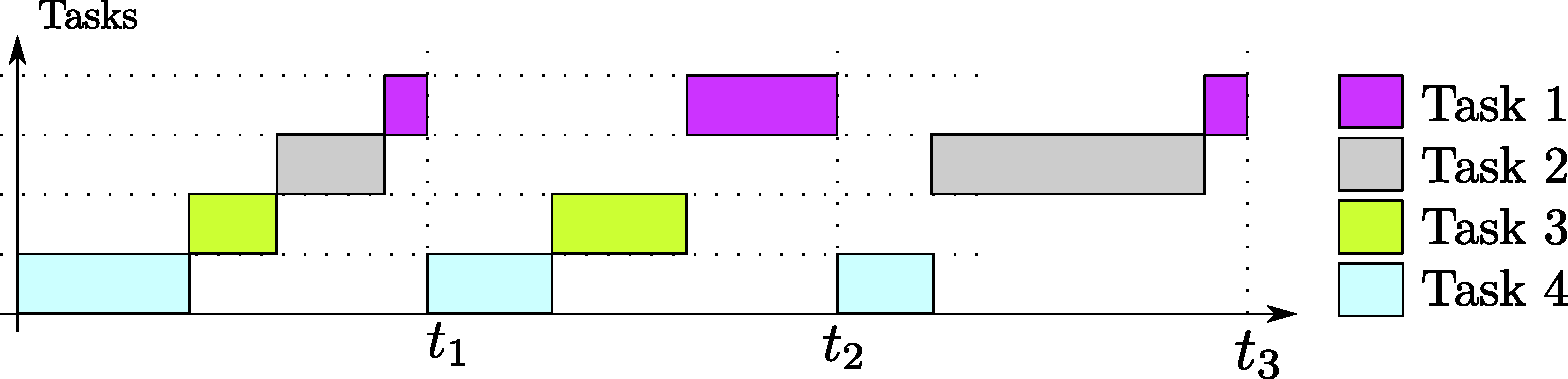
\includegraphics[scale=0.5]{figures/roundRobinSchedule2.pdf}
	\caption{Schedule with a shorter period than the time needed to process all the tasks}
	\label{roundRobinSchedule2}
\end{figure}

As the actual time to run the code is 2.8ms, and the sample time is 15ms, the prioritization of the tasks is not needed, because all the tasks will be ran at each sample.\\\\



The harware and Software choice have been explained, the sensors can now be implemented, independently from each other.